% This LaTeX was auto-generated from MATLAB code.
% To make changes, update the MATLAB code and export to LaTeX again.

\documentclass{article}

\usepackage[utf8]{inputenc}
\usepackage[T1]{fontenc}
\usepackage{lmodern}
\usepackage{graphicx}
\usepackage{color}
\usepackage{hyperref}
\usepackage{amsmath}
\usepackage{amsfonts}
\usepackage{epstopdf}
\usepackage[table]{xcolor}
\usepackage{matlab}
\usepackage[paperheight=795pt,paperwidth=614pt,top=72pt,bottom=72pt,right=72pt,left=72pt,heightrounded]{geometry}

\sloppy
\epstopdfsetup{outdir=./}
\graphicspath{ {./Pspeed_Rkin_media/} }

\begin{document}

\begin{matlabcode}
%% PREDICTORS: SPEED CONDITION, RESPONSE: KINEMATICS, STATS TEST
STATS_OUT = [];
im_resize= 1.2;
VIOLIN_BOTTOM = 0.7;
AX_H  = 0.2;
AX_W = 0.25;
DO_PLOT_GROUPS = false;
tmp_savedir = [save_dir filesep 'Pspeed-Rkin'];
mkdir(tmp_savedir);
\end{matlabcode}
\begin{matlaboutput}
Warning: Directory already exists.
\end{matlaboutput}
\begin{matlabcode}
for var_i = 1:length(varnames)
    %
    vert_shift = 0;
    for des_i = 2 %## JUST SPEED
        %##
        horiz_shift = 0;
        switch des_i
            case 1
                color_dark = COLORS_MAPS_TERRAIN;
                color_light = COLORS_MAPS_TERRAIN;
                GROUP_CMAP_OFFSET = [0,0.1,0.1];
                xtick_label_g = {'flat','low','med','high'};
            case 2
                color_dark = COLOR_MAPS_SPEED;
                color_light = COLOR_MAPS_SPEED+0.15;
                GROUP_CMAP_OFFSET = [0.15,0,0];
                xtick_label_g = {'0.25','0.50','0.75','1.0'};
        end
        inds = TMP_FOOOF_T.design_id == designs(des_i);
        T_vals_plot = TMP_FOOOF_T(inds,:);
        subjects = unique(T_vals_plot.subj_char);
        conds = unique(T_vals_plot.cond_id);
        % groups = unique(T_vals_plot.group_id);
        t_tmp = [];
        for i = 1:length(subjects)
            ii = find(T_vals_plot.subj_char == subjects(i));
            tt = T_vals_plot(ii,:);
            for j = 1:length(conds)
                jj = find(tt.cond_id == conds(j));
                t_tmp = [t_tmp; tt(jj(1),:)];
            end
        end
        T_vals_plot = table(categorical(string(t_tmp.cond_char)),t_tmp.(varnames{var_i}),categorical(string(t_tmp.group_char)),...
           'VariableNames',{'cond_char',varnames{var_i},'group_char'});
        % T_vals_plot.cond_char = double(string(T_vals_plot.cond_char));
        try
            mod = sprintf('%s ~ 1 + %s',varnames{var_i},'cond_char');
            % stats_out = fitlme(T_vals_plot,mod);
            stats_out = fitlm(T_vals_plot,mod);
            % anova_out = anova(stats_out);
            out = anova(T_vals_plot,mod,'SumOfSquaresType',"three",'CategoricalFactors',{'cond_char'},...
                'ModelSpecification','linear');
            anova_out = out.stats();
            % anova_out = anovan(double(T_vals_plot.(varnames{var_i})),{T_vals_plot.cond_char},...
            %             'model','linear',...
            %             'model',1,...
            %             'sstype',3,...
            %             'varnames',strvcat('speed'));

            %## PRINT TABLES
            t = sprintf_table(anova_out);
            % t.saveToFile([tmp_savedir filesep sprintf('%s_kinematics-speed_ANOVA.tex',varnames{var_i})]);
            t = sprintf_table(stats_out.Coefficients);
            % t.saveToFile([tmp_savedir filesep sprintf('%s_kinematics-speed_LM.tex',varnames{var_i})]);
            %-
            R2 = stats_out.Rsquared.Adjusted;
            anova_p_var = anova_out.pValue(strcmp(anova_out.Properties.RowNames,'cond_char'));
            pval_inter = double(stats_out.Coefficients.pValue(strcmp(stats_out.Coefficients.Properties.RowNames,'(Intercept)')));
            pval_var_0p5 = stats_out.Coefficients.pValue(strcmp(stats_out.Coefficients.Properties.RowNames,'cond_char_0.5'));
            pval_var_0p75 = stats_out.Coefficients.pValue(strcmp(stats_out.Coefficients.Properties.RowNames,'cond_char_0.75'));
            pval_var_1p0 = stats_out.Coefficients.pValue(strcmp(stats_out.Coefficients.Properties.RowNames,'cond_char_1.0'));
            % tstat_var = stats_out.Coefficients.tStat(strcmp(stats_out.Coefficients.Properties.RowNames,'cond_char'));
            % slope_var = double(stats_out.Coefficients.Estimate(strcmp(stats_out.Coefficients.Properties.RowNames,'cond_char')));
            inter_mn = double(stats_out.Coefficients.Estimate(strcmp(stats_out.Coefficients.Properties.RowNames,'(Intercept)')));
        catch e
            fprintf('Error. Cluster %s\n\n%s\n',string(clusters(cl_i)),getReport(e))
            R2 = 0;
            pval = 1;
            slope = 0;
            inter = 0;
        end
        %##
            STATS_STRUCT = struct('anova',{{}},...
                          'anova_grp',{{}},...
                          'pvals',{{}},...
                          'pvals_pairs',{{}},...
                          'pvals_grp',{{}},...
                          'pvals_grp_pairs',{{}},...
                          'regress_pval',{{}},...
                          'regress_line',{{}},...
                          'r2_coeff',{{}},...
                          'regress_xvals',0);
        if DO_PLOT_GROUPS
            for gg = 1:length(groups)
                STATS_STRUCT.anova{gg}=anova_p_var;
                STATS_STRUCT.pvals_pairs{gg}={[1,1],[1,2],[1,3],[1,4]};
                STATS_STRUCT.pvals{gg}=[pval_inter,pval_var_0p5,pval_var_0p75,pval_var_1p0];
            end
        else
            STATS_STRUCT.anova{1}=anova_p_var;
            STATS_STRUCT.pvals_pairs{1}={[1,1],[1,2],[1,3],[1,4]};
            STATS_STRUCT.pvals{1}=[pval_inter,pval_var_0p5,pval_var_0p75,pval_var_1p0];
        end
        STATS_OUT = [STATS_OUT; STATS_STRUCT];
        % figure;
        VIOLIN_PARAMS = {'width',0.1,...
            'ShowWhiskers',false,'ShowNotches',false,'ShowBox',true,...
            'ShowMedian',true,'Bandwidth',0.15,'QuartileStyle','shadow',...
            'HalfViolin','full','DataStyle','scatter','MarkerSize',8,...
            'EdgeColor',[0.5,0.5,0.5],'ViolinAlpha',{0.2 0.3}};
        PLOT_PARAMS = struct('color_map',color_dark,...
            'cond_labels',unique(T_vals_plot.cond_char),'group_labels',unique(T_vals_plot.group_char),...
            'cond_offsets',[-0.35,-0.1,0.15,0.4],'y_label',varnames_labs{var_i},...
            'title',varnames_labs{var_i},'font_size',10,'group_offsets',[0.125,0.475,0.812],...
            'ylim',[min(T_vals_plot.(varnames{var_i}))-std(T_vals_plot.(varnames{var_i})),max(T_vals_plot.(varnames{var_i}))+3*std(T_vals_plot.(varnames{var_i}))],...
            'font_name','Arial','x_label','speed','do_combine_groups',~DO_PLOT_GROUPS);
        fig = figure('color','white','renderer','Painters');
        set(fig,'Units','inches','Position',[0.5,0.5,6.5,9])
        set(fig,'PaperUnits','inches','PaperSize',[1 1],'PaperPosition',[0 0 1 1])
        hold on;
        set(gca,AXES_DEFAULT_PROPS{:})
        axax = group_violin(T_vals_plot,varnames{var_i},'cond_char','group_char',...
            fig,...
            'VIOLIN_PARAMS',VIOLIN_PARAMS,...
            'PLOT_PARAMS',PLOT_PARAMS,...
            'STATS_STRUCT',STATS_STRUCT);
        set(axax,'OuterPosition',[0,0,1,1]);
        set(axax,'Position',[0.1+horiz_shift,VIOLIN_BOTTOM+vert_shift,AX_W*im_resize,AX_H*im_resize]);  %[left bottom width height]
        hold off;
        exportgraphics(fig,[tmp_savedir filesep sprintf('%s_kinematics-speed-factor_grouped.tiff',varnames{var_i})],'Resolution',300)
        % exportgraphics(fig,[tmp_savedir filesep sprintf('%s_kinematics-speed-contin_grouped.tiff',varnames{var_i})],'Resolution',300)
        close(fig)
        %- iterate
   end
end
\end{matlabcode}
\begin{matlaboutput}
% PrintTable generated on 24-Apr-2024 11:28:14
% Created in sprintf_table:17 at M:\jsalminen\GitHub\par_EEGProcessing\src\_functions\v2_0\sprintf_table.m
% Export settings: TexMathModeDetection 1, HasHeader 1, HasRowHeader 0, StripInsertedTabChars 1, IsPDF 0, TightPDF 1
\begin{table}[!hb]
	\centering
	\def\arraystretch{1.3}
	\begin{tabular}{llllll}
				& SumOfSquares	& DF	& MeanSquares	& F		& pValue\\
		\hline\\
		cond_char	& $519.328$	& $3$	& $173.109$	& $4.03328$	& $0.00770893$\\
		Error		& $14592.9$	& $340$	& $42.9202$	& NaN		& NaN\\
		Total		& $15112.2$	& $343$	& NaN		& NaN		& NaN\\
	\end{tabular}
\end{table}
% PrintTable generated on 24-Apr-2024 11:28:14
% Created in sprintf_table:17 at M:\jsalminen\GitHub\par_EEGProcessing\src\_functions\v2_0\sprintf_table.m
% Export settings: TexMathModeDetection 1, HasHeader 1, HasRowHeader 0, StripInsertedTabChars 1, IsPDF 0, TightPDF 1
\begin{table}[!hb]
	\centering
	\def\arraystretch{1.3}
	\begin{tabular}{lllll}
				& Estimate	& SE		& tStat		& pValue\\
		\hline\\
		(Intercept)	& $22.722$	& $0.706451$	& $32.1635$	& $0$\\
		cond_char_0.5	& $-2.07218$	& $0.999072$	& $-2.0741$	& $0.0388218$\\
		cond_char_0.75	& $-2.82728$	& $0.999072$	& $-2.8299$	& $0.00493286$\\
		cond_char_1.0	& $-3.16191$	& $0.999072$	& $-3.16485$	& $0.00169179$\\
	\end{tabular}
\end{table}
Condition 0.25 & Group 1 does not have outliers
lbl = '*'
\end{matlaboutput}
\begin{center}
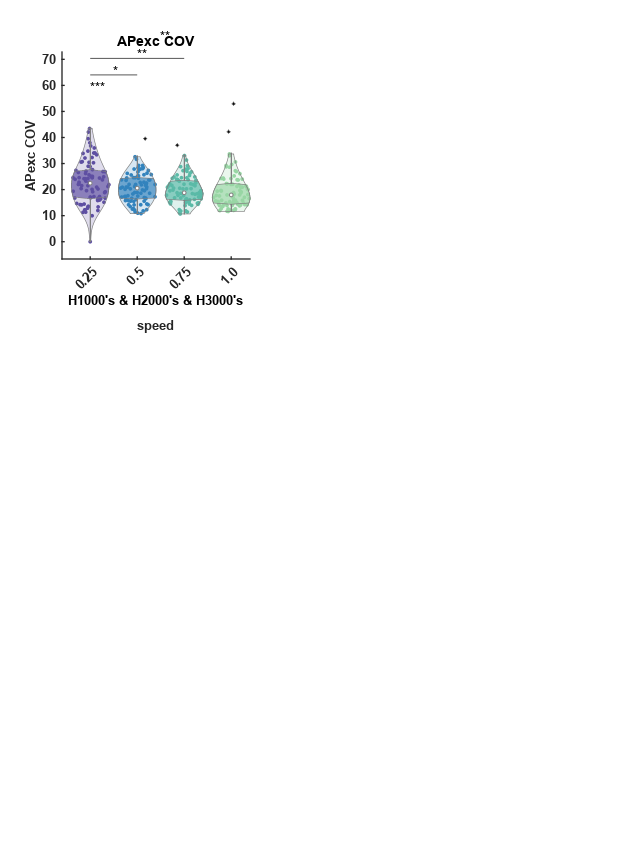
\includegraphics[width=\maxwidth{62.61916708479679em}]{figure_0.png}
\end{center}
\begin{matlaboutput}
% PrintTable generated on 24-Apr-2024 11:28:16
% Created in sprintf_table:17 at M:\jsalminen\GitHub\par_EEGProcessing\src\_functions\v2_0\sprintf_table.m
% Export settings: TexMathModeDetection 1, HasHeader 1, HasRowHeader 0, StripInsertedTabChars 1, IsPDF 0, TightPDF 1
\begin{table}[!hb]
	\centering
	\def\arraystretch{1.3}
	\begin{tabular}{llllll}
				& SumOfSquares	& DF	& MeanSquares	& F		& pValue\\
		\hline\\
		cond_char	& $0.0251355$	& $3$	& $0.0083785$	& $43.5204$	& $7.94633e-24$\\
		Error		& $0.0654564$	& $340$	& $0.000192519$	& NaN		& NaN\\
		Total		& $0.0905919$	& $343$	& NaN		& NaN		& NaN\\
	\end{tabular}
\end{table}
% PrintTable generated on 24-Apr-2024 11:28:16
% Created in sprintf_table:17 at M:\jsalminen\GitHub\par_EEGProcessing\src\_functions\v2_0\sprintf_table.m
% Export settings: TexMathModeDetection 1, HasHeader 1, HasRowHeader 0, StripInsertedTabChars 1, IsPDF 0, TightPDF 1
\begin{table}[!hb]
	\centering
	\def\arraystretch{1.3}
	\begin{tabular}{lllll}
				& Estimate	& SE		& tStat		& pValue\\
		\hline\\
		(Intercept)	& $0.0600316$	& $0.00149619$	& $40.1229$	& $0$\\
		cond_char_0.5	& $-0.0108131$	& $0.00211594$	& $-5.11031$	& $5.37553e-07$\\
		cond_char_0.75	& $-0.0185562$	& $0.00211594$	& $-8.76975$	& $1.11022e-16$\\
		cond_char_1.0	& $-0.0223615$	& $0.00211594$	& $-10.5681$	& $0$\\
	\end{tabular}
\end{table}
Condition 0.25 & Group 1 does not have outliers
Condition 0.5 & Group 1 does not have outliers
Condition 0.75 & Group 1 does not have outliers
\end{matlaboutput}
\begin{center}
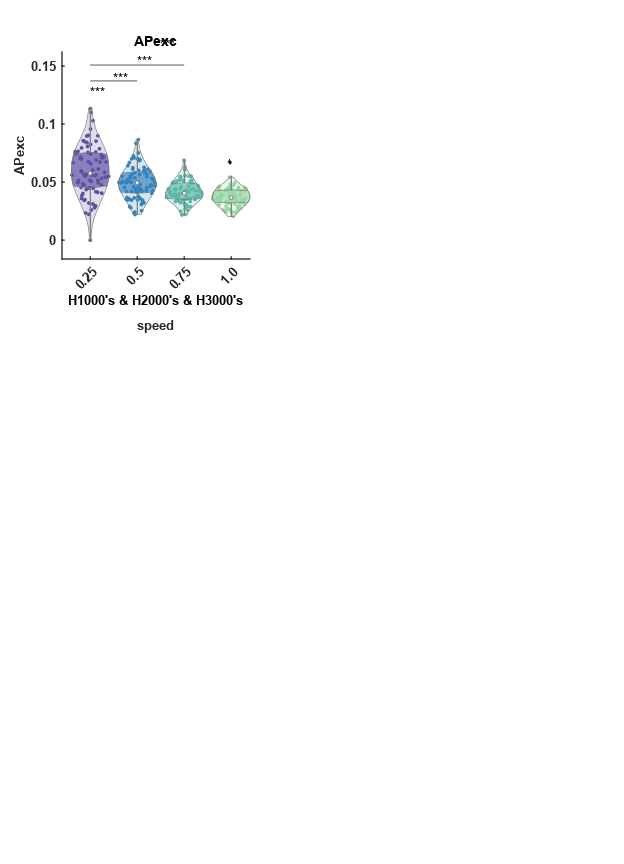
\includegraphics[width=\maxwidth{62.61916708479679em}]{figure_1.png}
\end{center}
\begin{matlaboutput}
% PrintTable generated on 24-Apr-2024 11:28:19
% Created in sprintf_table:17 at M:\jsalminen\GitHub\par_EEGProcessing\src\_functions\v2_0\sprintf_table.m
% Export settings: TexMathModeDetection 1, HasHeader 1, HasRowHeader 0, StripInsertedTabChars 1, IsPDF 0, TightPDF 1
\begin{table}[!hb]
	\centering
	\def\arraystretch{1.3}
	\begin{tabular}{llllll}
				& SumOfSquares	& DF	& MeanSquares	& F		& pValue\\
		\hline\\
		cond_char	& $1329.22$	& $3$	& $443.072$	& $20.231$	& $4.35657e-12$\\
		Error		& $7446.21$	& $340$	& $21.9006$	& NaN		& NaN\\
		Total		& $8775.43$	& $343$	& NaN		& NaN		& NaN\\
	\end{tabular}
\end{table}
% PrintTable generated on 24-Apr-2024 11:28:19
% Created in sprintf_table:17 at M:\jsalminen\GitHub\par_EEGProcessing\src\_functions\v2_0\sprintf_table.m
% Export settings: TexMathModeDetection 1, HasHeader 1, HasRowHeader 0, StripInsertedTabChars 1, IsPDF 0, TightPDF 1
\begin{table}[!hb]
	\centering
	\def\arraystretch{1.3}
	\begin{tabular}{lllll}
				& Estimate	& SE		& tStat		& pValue\\
		\hline\\
		(Intercept)	& $12.0448$	& $0.504637$	& $23.8683$	& $0$\\
		cond_char_0.5	& $0.587023$	& $0.713664$	& $0.822547$	& $0.411342$\\
		cond_char_0.75	& $2.51273$	& $0.713664$	& $3.52089$	& $0.000488732$\\
		cond_char_1.0	& $5.03332$	& $0.713664$	& $7.05278$	& $9.86178e-12$\\
	\end{tabular}
\end{table}
Condition 1.0 & Group 1 does not have outliers
\end{matlaboutput}
\begin{center}
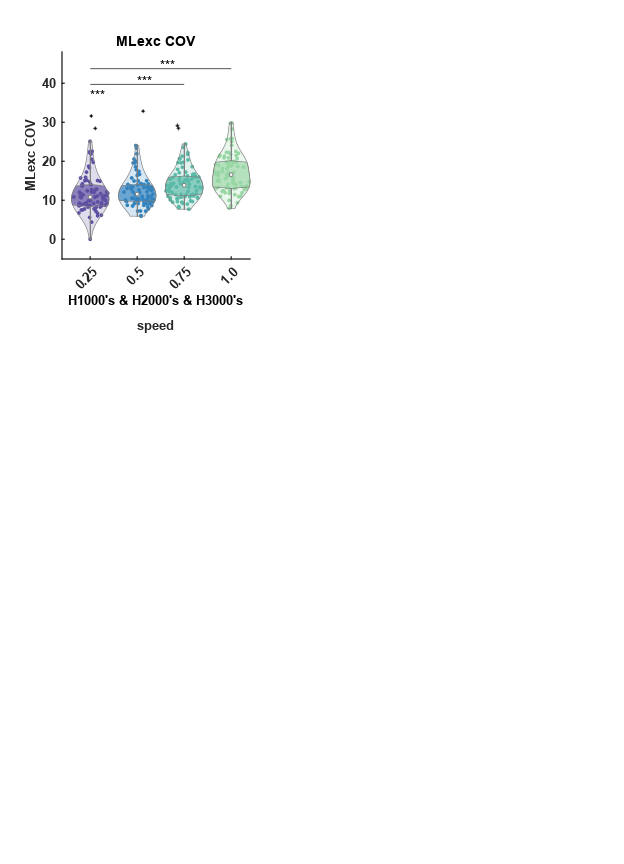
\includegraphics[width=\maxwidth{62.61916708479679em}]{figure_2.png}
\end{center}
\begin{matlaboutput}
% PrintTable generated on 24-Apr-2024 11:28:22
% Created in sprintf_table:17 at M:\jsalminen\GitHub\par_EEGProcessing\src\_functions\v2_0\sprintf_table.m
% Export settings: TexMathModeDetection 1, HasHeader 1, HasRowHeader 0, StripInsertedTabChars 1, IsPDF 0, TightPDF 1
\begin{table}[!hb]
	\centering
	\def\arraystretch{1.3}
	\begin{tabular}{llllll}
				& SumOfSquares	& DF	& MeanSquares	& F		& pValue\\
		\hline\\
		cond_char	& $0.202518$	& $3$	& $0.0675058$	& $111.936$	& $1.99328e-50$\\
		Error		& $0.205046$	& $340$	& $0.000603076$	& NaN		& NaN\\
		Total		& $0.407564$	& $343$	& NaN		& NaN		& NaN\\
	\end{tabular}
\end{table}
% PrintTable generated on 24-Apr-2024 11:28:22
% Created in sprintf_table:17 at M:\jsalminen\GitHub\par_EEGProcessing\src\_functions\v2_0\sprintf_table.m
% Export settings: TexMathModeDetection 1, HasHeader 1, HasRowHeader 0, StripInsertedTabChars 1, IsPDF 0, TightPDF 1
\begin{table}[!hb]
	\centering
	\def\arraystretch{1.3}
	\begin{tabular}{lllll}
				& Estimate	& SE		& tStat		& pValue\\
		\hline\\
		(Intercept)	& $0.120388$	& $0.00264812$	& $45.4618$	& $0$\\
		cond_char_0.5	& $-0.0258579$	& $0.003745$	& $-6.90464$	& $2.47975e-11$\\
		cond_char_0.75	& $-0.0493465$	& $0.003745$	& $-13.1766$	& $0$\\
		cond_char_1.0	& $-0.0639934$	& $0.003745$	& $-17.0877$	& $0$\\
	\end{tabular}
\end{table}
Condition 0.75 & Group 1 does not have outliers
\end{matlaboutput}
\begin{center}
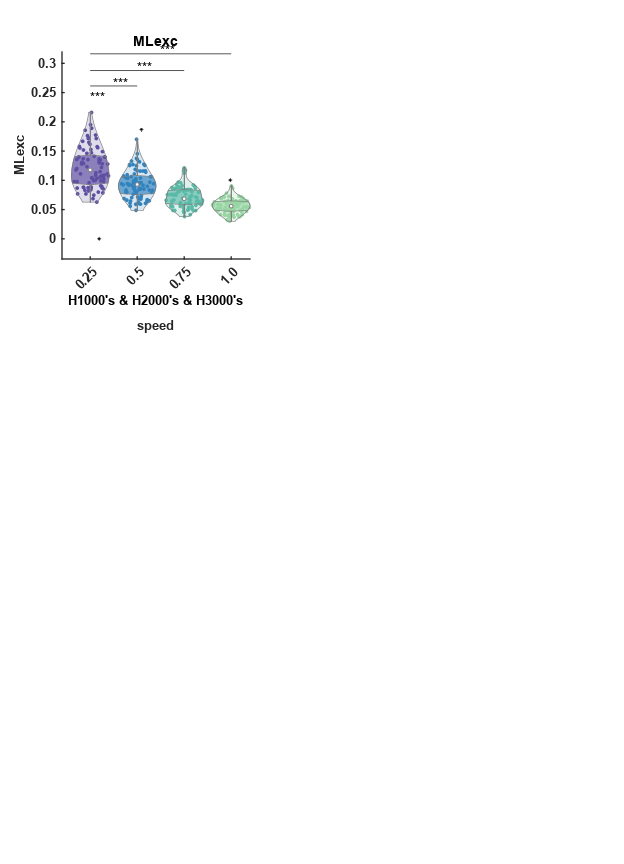
\includegraphics[width=\maxwidth{62.61916708479679em}]{figure_3.png}
\end{center}
\begin{matlaboutput}
% PrintTable generated on 24-Apr-2024 11:28:25
% Created in sprintf_table:17 at M:\jsalminen\GitHub\par_EEGProcessing\src\_functions\v2_0\sprintf_table.m
% Export settings: TexMathModeDetection 1, HasHeader 1, HasRowHeader 0, StripInsertedTabChars 1, IsPDF 0, TightPDF 1
\begin{table}[!hb]
	\centering
	\def\arraystretch{1.3}
	\begin{tabular}{llllll}
				& SumOfSquares	& DF	& MeanSquares	& F		& pValue\\
		\hline\\
		cond_char	& $15.5399$	& $3$	& $5.17997$	& $206.85$	& $2.49716e-76$\\
		Error		& $8.51432$	& $340$	& $0.0250421$	& NaN		& NaN\\
		Total		& $24.0542$	& $343$	& NaN		& NaN		& NaN\\
	\end{tabular}
\end{table}
% PrintTable generated on 24-Apr-2024 11:28:25
% Created in sprintf_table:17 at M:\jsalminen\GitHub\par_EEGProcessing\src\_functions\v2_0\sprintf_table.m
% Export settings: TexMathModeDetection 1, HasHeader 1, HasRowHeader 0, StripInsertedTabChars 1, IsPDF 0, TightPDF 1
\begin{table}[!hb]
	\centering
	\def\arraystretch{1.3}
	\begin{tabular}{lllll}
				& Estimate	& SE		& tStat		& pValue\\
		\hline\\
		(Intercept)	& $1.1361$	& $0.0170642$	& $66.5778$	& $0$\\
		cond_char_0.5	& $-0.337826$	& $0.0241324$	& $-13.9988$	& $0$\\
		cond_char_0.75	& $-0.477066$	& $0.0241324$	& $-19.7687$	& $0$\\
		cond_char_1.0	& $-0.555245$	& $0.0241324$	& $-23.0082$	& $0$\\
	\end{tabular}
\end{table}
Condition 0.25 & Group 1 does not have outliers
Condition 0.5 & Group 1 does not have outliers
Condition 0.75 & Group 1 does not have outliers
\end{matlaboutput}
\begin{center}
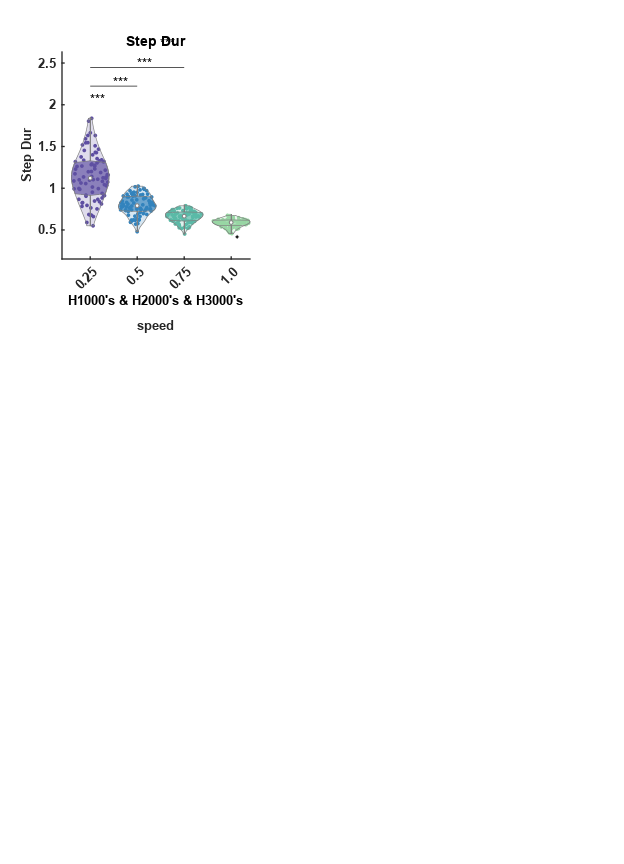
\includegraphics[width=\maxwidth{62.61916708479679em}]{figure_4.png}
\end{center}
\begin{matlaboutput}
% PrintTable generated on 24-Apr-2024 11:28:28
% Created in sprintf_table:17 at M:\jsalminen\GitHub\par_EEGProcessing\src\_functions\v2_0\sprintf_table.m
% Export settings: TexMathModeDetection 1, HasHeader 1, HasRowHeader 0, StripInsertedTabChars 1, IsPDF 0, TightPDF 1
\begin{table}[!hb]
	\centering
	\def\arraystretch{1.3}
	\begin{tabular}{llllll}
				& SumOfSquares	& DF	& MeanSquares	& F		& pValue\\
		\hline\\
		cond_char	& $6713.83$	& $3$	& $2237.94$	& $199.697$	& $1.15557e-74$\\
		Error		& $3810.27$	& $340$	& $11.2067$	& NaN		& NaN\\
		Total		& $10524.1$	& $343$	& NaN		& NaN		& NaN\\
	\end{tabular}
\end{table}
% PrintTable generated on 24-Apr-2024 11:28:28
% Created in sprintf_table:17 at M:\jsalminen\GitHub\par_EEGProcessing\src\_functions\v2_0\sprintf_table.m
% Export settings: TexMathModeDetection 1, HasHeader 1, HasRowHeader 0, StripInsertedTabChars 1, IsPDF 0, TightPDF 1
\begin{table}[!hb]
	\centering
	\def\arraystretch{1.3}
	\begin{tabular}{lllll}
				& Estimate	& SE		& tStat		& pValue\\
		\hline\\
		(Intercept)	& $19.9955$	& $0.360985$	& $55.3914$	& $0$\\
		cond_char_0.5	& $-5.61592$	& $0.51051$	& $-11.0006$	& $0$\\
		cond_char_0.75	& $-9.37972$	& $0.51051$	& $-18.3732$	& $0$\\
		cond_char_1.0	& $-11.6825$	& $0.51051$	& $-22.884$	& $0$\\
	\end{tabular}
\end{table}
Condition 0.5 & Group 1 does not have outliers
Condition 0.75 & Group 1 does not have outliers
\end{matlaboutput}
\begin{center}
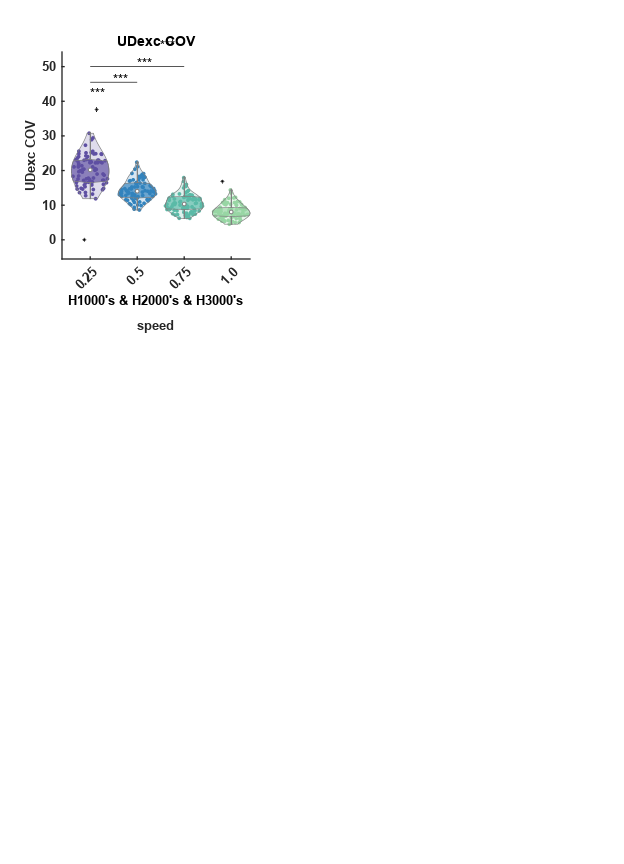
\includegraphics[width=\maxwidth{62.61916708479679em}]{figure_5.png}
\end{center}
\begin{matlaboutput}
% PrintTable generated on 24-Apr-2024 11:28:30
% Created in sprintf_table:17 at M:\jsalminen\GitHub\par_EEGProcessing\src\_functions\v2_0\sprintf_table.m
% Export settings: TexMathModeDetection 1, HasHeader 1, HasRowHeader 0, StripInsertedTabChars 1, IsPDF 0, TightPDF 1
\begin{table}[!hb]
	\centering
	\def\arraystretch{1.3}
	\begin{tabular}{llllll}
				& SumOfSquares	& DF	& MeanSquares	& F		& pValue\\
		\hline\\
		cond_char	& $0.0207407$	& $3$	& $0.00691357$	& $228.604$	& $3.56272e-81$\\
		Error		& $0.0102825$	& $340$	& $3.02426e-05$	& NaN		& NaN\\
		Total		& $0.0310232$	& $343$	& NaN		& NaN		& NaN\\
	\end{tabular}
\end{table}
% PrintTable generated on 24-Apr-2024 11:28:31
% Created in sprintf_table:17 at M:\jsalminen\GitHub\par_EEGProcessing\src\_functions\v2_0\sprintf_table.m
% Export settings: TexMathModeDetection 1, HasHeader 1, HasRowHeader 0, StripInsertedTabChars 1, IsPDF 0, TightPDF 1
\begin{table}[!hb]
	\centering
	\def\arraystretch{1.3}
	\begin{tabular}{lllll}
				& Estimate	& SE		& tStat		& pValue\\
		\hline\\
		(Intercept)	& $0.0147353$	& $0.000593008$	& $24.8484$	& $0$\\
		cond_char_0.5	& $0.00508205$	& $0.000838639$	& $6.05988$	& $3.61574e-09$\\
		cond_char_0.75	& $0.0121604$	& $0.000838639$	& $14.5002$	& $0$\\
		cond_char_1.0	& $0.0206502$	& $0.000838639$	& $24.6235$	& $0$\\
	\end{tabular}
\end{table}
Condition 1.0 & Group 1 does not have outliers
\end{matlaboutput}
\begin{center}
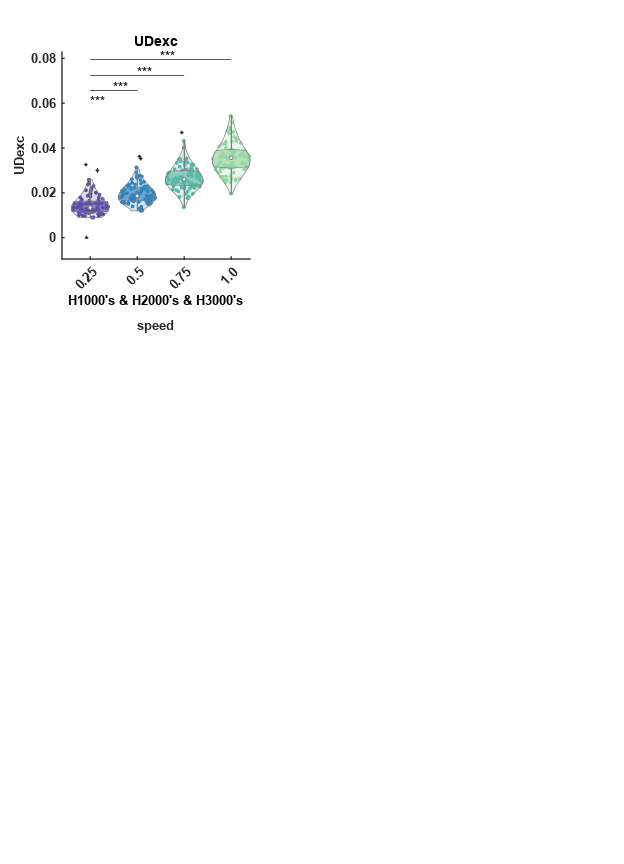
\includegraphics[width=\maxwidth{62.61916708479679em}]{figure_6.png}
\end{center}
\begin{matlaboutput}
% PrintTable generated on 24-Apr-2024 11:28:33
% Created in sprintf_table:17 at M:\jsalminen\GitHub\par_EEGProcessing\src\_functions\v2_0\sprintf_table.m
% Export settings: TexMathModeDetection 1, HasHeader 1, HasRowHeader 0, StripInsertedTabChars 1, IsPDF 0, TightPDF 1
\begin{table}[!hb]
	\centering
	\def\arraystretch{1.3}
	\begin{tabular}{llllll}
				& SumOfSquares	& DF	& MeanSquares	& F		& pValue\\
		\hline\\
		cond_char	& $45.3796$	& $3$	& $15.1265$	& $265.163$	& $1.15424e-88$\\
		Error		& $19.3957$	& $340$	& $0.0570463$	& NaN		& NaN\\
		Total		& $64.7753$	& $343$	& NaN		& NaN		& NaN\\
	\end{tabular}
\end{table}
% PrintTable generated on 24-Apr-2024 11:28:33
% Created in sprintf_table:17 at M:\jsalminen\GitHub\par_EEGProcessing\src\_functions\v2_0\sprintf_table.m
% Export settings: TexMathModeDetection 1, HasHeader 1, HasRowHeader 0, StripInsertedTabChars 1, IsPDF 0, TightPDF 1
\begin{table}[!hb]
	\centering
	\def\arraystretch{1.3}
	\begin{tabular}{lllll}
				& Estimate	& SE		& tStat		& pValue\\
		\hline\\
		(Intercept)	& $1.67033$	& $0.0257552$	& $64.8541$	& $0$\\
		cond_char_0.5	& $-0.603103$	& $0.0364233$	& $-16.5582$	& $0$\\
		cond_char_0.75	& $-0.825342$	& $0.0364233$	& $-22.6597$	& $0$\\
		cond_char_1.0	& $-0.942194$	& $0.0364233$	& $-25.8679$	& $0$\\
	\end{tabular}
\end{table}
Condition 0.25 & Group 1 does not have outliers
Condition 0.5 & Group 1 does not have outliers
Condition 0.75 & Group 1 does not have outliers
\end{matlaboutput}
\begin{center}
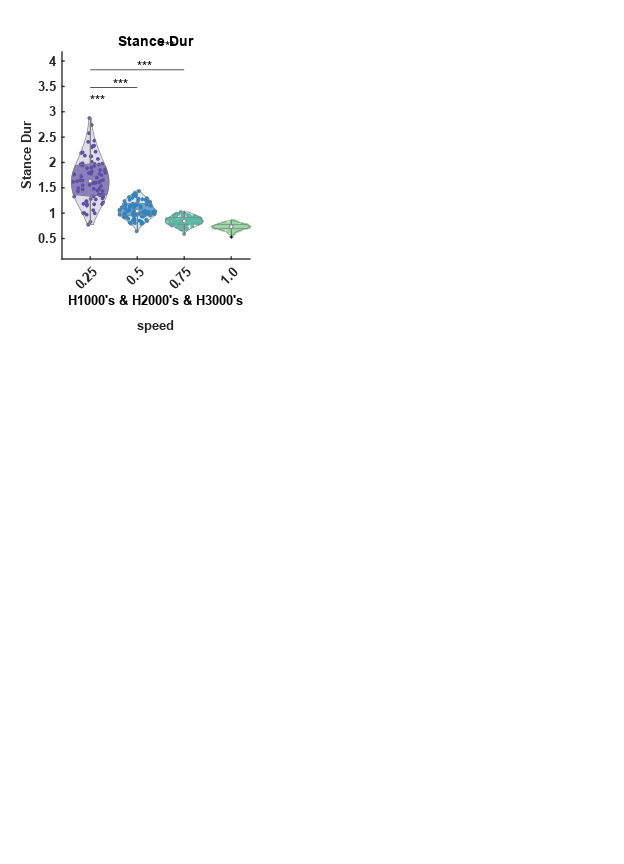
\includegraphics[width=\maxwidth{62.61916708479679em}]{figure_7.png}
\end{center}
\begin{matlaboutput}
% PrintTable generated on 24-Apr-2024 11:28:36
% Created in sprintf_table:17 at M:\jsalminen\GitHub\par_EEGProcessing\src\_functions\v2_0\sprintf_table.m
% Export settings: TexMathModeDetection 1, HasHeader 1, HasRowHeader 0, StripInsertedTabChars 1, IsPDF 0, TightPDF 1
\begin{table}[!hb]
	\centering
	\def\arraystretch{1.3}
	\begin{tabular}{llllll}
				& SumOfSquares	& DF	& MeanSquares	& F		& pValue\\
		\hline\\
		cond_char	& $62.421$	& $3$	& $20.807$	& $207.088$	& $2.20199e-76$\\
		Error		& $34.1613$	& $340$	& $0.100474$	& NaN		& NaN\\
		Total		& $96.5824$	& $343$	& NaN		& NaN		& NaN\\
	\end{tabular}
\end{table}
% PrintTable generated on 24-Apr-2024 11:28:36
% Created in sprintf_table:17 at M:\jsalminen\GitHub\par_EEGProcessing\src\_functions\v2_0\sprintf_table.m
% Export settings: TexMathModeDetection 1, HasHeader 1, HasRowHeader 0, StripInsertedTabChars 1, IsPDF 0, TightPDF 1
\begin{table}[!hb]
	\centering
	\def\arraystretch{1.3}
	\begin{tabular}{lllll}
				& Estimate	& SE		& tStat		& pValue\\
		\hline\\
		(Intercept)	& $2.27456$	& $0.0341805$	& $66.5454$	& $0$\\
		cond_char_0.5	& $-0.677493$	& $0.0483386$	& $-14.0156$	& $0$\\
		cond_char_0.75	& $-0.956365$	& $0.0483386$	& $-19.7847$	& $0$\\
		cond_char_1.0	& $-1.11269$	& $0.0483386$	& $-23.0186$	& $0$\\
	\end{tabular}
\end{table}
Condition 0.25 & Group 1 does not have outliers
Condition 0.5 & Group 1 does not have outliers
Condition 0.75 & Group 1 does not have outliers
\end{matlaboutput}
\begin{center}
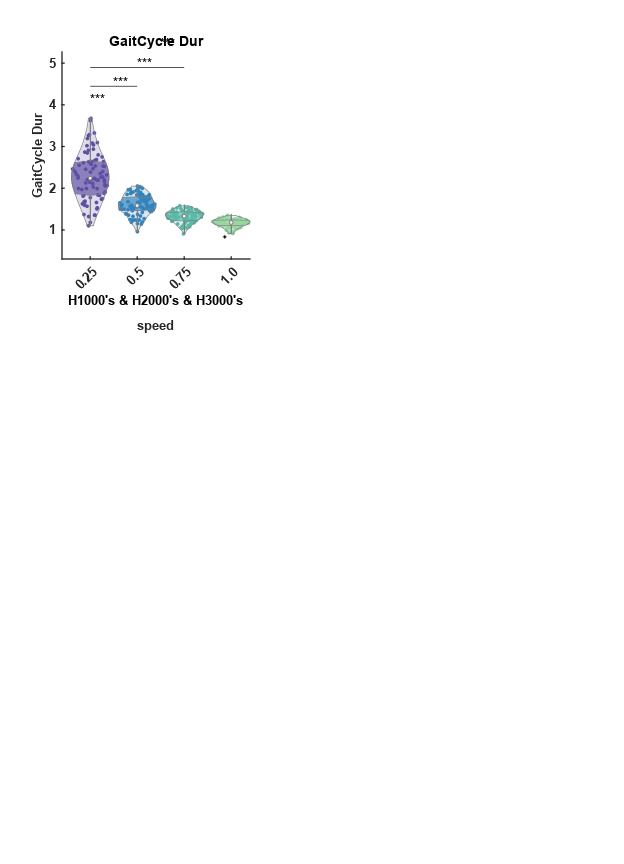
\includegraphics[width=\maxwidth{62.61916708479679em}]{figure_8.png}
\end{center}
\begin{matlaboutput}
% PrintTable generated on 24-Apr-2024 11:28:38
% Created in sprintf_table:17 at M:\jsalminen\GitHub\par_EEGProcessing\src\_functions\v2_0\sprintf_table.m
% Export settings: TexMathModeDetection 1, HasHeader 1, HasRowHeader 0, StripInsertedTabChars 1, IsPDF 0, TightPDF 1
\begin{table}[!hb]
	\centering
	\def\arraystretch{1.3}
	\begin{tabular}{llllll}
				& SumOfSquares	& DF	& MeanSquares	& F		& pValue\\
		\hline\\
		cond_char	& $3.84599$	& $3$	& $1.282$	& $453.704$	& $1.76735e-118$\\
		Error		& $0.960712$	& $340$	& $0.00282562$	& NaN		& NaN\\
		Total		& $4.80671$	& $343$	& NaN		& NaN		& NaN\\
	\end{tabular}
\end{table}
% PrintTable generated on 24-Apr-2024 11:28:38
% Created in sprintf_table:17 at M:\jsalminen\GitHub\par_EEGProcessing\src\_functions\v2_0\sprintf_table.m
% Export settings: TexMathModeDetection 1, HasHeader 1, HasRowHeader 0, StripInsertedTabChars 1, IsPDF 0, TightPDF 1
\begin{table}[!hb]
	\centering
	\def\arraystretch{1.3}
	\begin{tabular}{lllll}
				& Estimate	& SE		& tStat		& pValue\\
		\hline\\
		(Intercept)	& $0.115701$	& $0.00573202$	& $20.185$	& $0$\\
		cond_char_0.5	& $0.082687$	& $0.00810631$	& $10.2003$	& $0$\\
		cond_char_0.75	& $0.172853$	& $0.00810631$	& $21.3233$	& $0$\\
		cond_char_1.0	& $0.28442$	& $0.00810631$	& $35.0863$	& $0$\\
	\end{tabular}
\end{table}
Condition 0.75 & Group 1 does not have outliers
Condition 1.0 & Group 1 does not have outliers
\end{matlaboutput}
\begin{center}
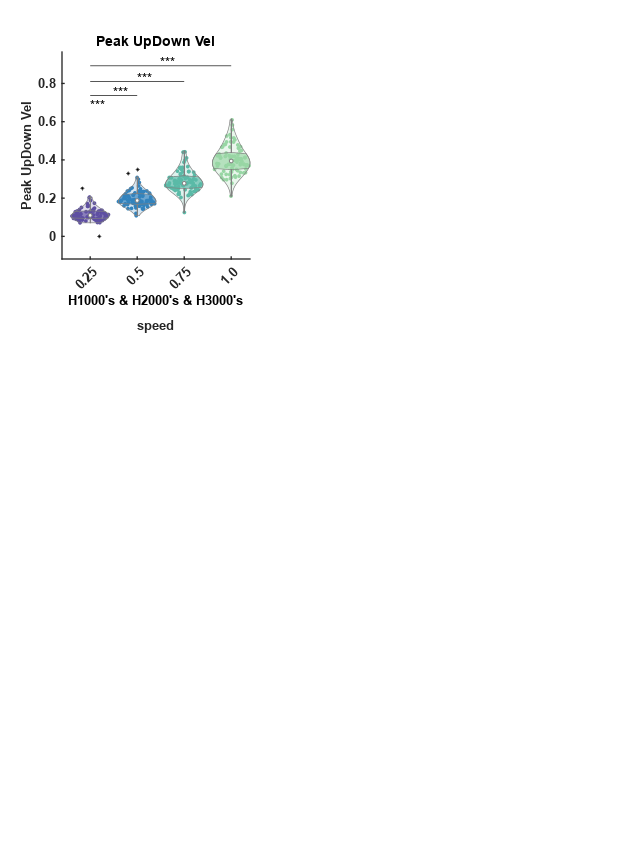
\includegraphics[width=\maxwidth{62.61916708479679em}]{figure_9.png}
\end{center}

\end{document}
